\documentclass[11pt,a4paper]{article}

\usepackage[utf8]{inputenc}
\usepackage[T1]{fontenc}
\usepackage[margin=2.2cm]{geometry}
\usepackage{parskip}
\usepackage{titlesec}
\usepackage{enumitem}
\usepackage{booktabs}
\usepackage{xcolor}
\usepackage{tcolorbox}
\usepackage{graphicx}
\usepackage{hyperref}
\usepackage{fancyhdr}
\usepackage{listings}
\usepackage{longtable}
\usepackage{array}

\tcbuselibrary{skins,breakable}

\renewcommand{\contentsname}{Contenido}
\renewcommand{\figurename}{Figura}

\definecolor{accent}{RGB}{30,80,150}
\definecolor{softgray}{RGB}{245,246,248}
\definecolor{codebg}{RGB}{248,248,250}
\definecolor{warn}{RGB}{160,60,40}
\definecolor{good}{RGB}{30,120,70}

\titleformat{\section}{\Large\bfseries\color{accent}}{\thesection}{0.8em}{}
\titleformat{\subsection}{\large\bfseries}{\thesubsection}{0.6em}{}

\hypersetup{colorlinks=true, linkcolor=accent, urlcolor=accent,
  pdftitle={AgentIA --- Informe Final},
  pdfauthor={Ingeniería AgentIA}}

\pagestyle{fancy}
\fancyhf{}
\fancyhead[L]{\small\color{accent}AgentIA --- Informe Final}
\fancyhead[R]{\small\color{accent}\thepage}
\renewcommand{\headrulewidth}{0.4pt}

\lstset{
  basicstyle=\ttfamily\small, backgroundcolor=\color{codebg},
  frame=single, rulecolor=\color{softgray}, breaklines=true,
  columns=fullflexible, keepspaces=true, showstringspaces=false,
  xleftmargin=0.4em, xrightmargin=0.4em,
}

\newtcolorbox{notebox}[1][]{colback=softgray,colframe=accent,boxrule=0.4pt,
  arc=2pt,left=6pt,right=6pt,top=4pt,bottom=4pt,breakable,#1}
\newtcolorbox{painbox}[1][]{colback=softgray,colframe=warn,boxrule=0.4pt,
  arc=2pt,left=6pt,right=6pt,top=4pt,bottom=4pt,breakable,#1}

\title{\vspace{-1.4cm}\textbf{AgentIA --- Informe Final}\\[0.25cm]
\large Del dolor al estado actual: la propuesta, la auto-mejora, el diseño guiado por
especificación, la orquestación, la interfaz y el coste}
\author{Ingeniería AgentIA}
\date{2026-09-29}

\begin{document}
\maketitle
\thispagestyle{fancy}

\tableofcontents
\vspace{0.4cm}

\section{El dolor}

Generar un microservicio de producción es caro, lento e inconsistente. Cada servicio
debe obedecer las mismas reglas --- capas estrictas, contratos inmutables, errores
centralizados, compilación hermética --- y cada incumplimiento se paga en revisión
humana, en defectos en producción o en deuda técnica. El problema no es escribir
código; es garantizar que el código cumple un estándar, de forma repetible y auditable.

\begin{painbox}
\textbf{El síntoma que lo hizo tangible.} Durante meses la plataforma reportó
\textbf{``0 de 15 sesiones verificadas''}: no podía demostrar que su propia salida
compilaba. La causa resultó ser un defecto de montaje Docker de un solo carácter, no
una limitación del generador. Un sistema que no puede verificar su propia salida no
puede prometer fiabilidad --- y esa era exactamente la brecha de producto.
\end{painbox}

\section{La propuesta}

\textbf{Microservice Code Studio}: un agente autónomo que convierte una especificación
formal en un microservicio Spring Boot completo, compilado y probado, y que se niega a
reportar éxito salvo que eso sea cierto.

\begin{center}
\begin{tabular}{@{}p{0.28\textwidth}p{0.66\textwidth}@{}}
\toprule
\textbf{Entrada} & una especificación formal (blueprint): entidades, atributos,
validaciones, historias BDD, arquitectura en 4 capas \\
\textbf{Generación} & un agente LangGraph de ocho etapas, gobernado por una compuerta
de cumplimiento determinista \\
\textbf{Verificación} & \texttt{mvn test -o} en un contenedor Docker hermético sin red,
con un test de contrato que el modelo no puede autorar \\
\textbf{Reparación} & auto-reparación acotada (máx.\ 3 intentos); al límite, \texttt{BLOQUEADO}
y pasa a humano \\
\textbf{Entrega} & descarga ZIP o publicación atómica a Git \\
\bottomrule
\end{tabular}
\end{center}

La promesa no es ``código mejor''; es \textbf{gobernanza}: el código cumple las reglas
del proyecto, verificado de forma determinista, a un coste predecible.

\section{La propuesta de auto-mejora}

Sobre el generador se propuso un bucle de auto-mejora reflexiva: un LLM reflexiona
sobre los diagnósticos registrados y propone ediciones a un documento de
``habilidad''; una edición se admite solo si su contribución medida es positiva, y se
desaloja solo si cae por debajo de un suelo de evidencia. Sin pesos, sin GPUs, sin
entrenamiento.

\begin{notebox}
\textbf{La condición que lo gobierna.} La literatura y la medición propia coinciden:
\textbf{un bucle alimentado solo con un veredicto binario no es mejor que ningún
bucle} (CoEvoSkills: 41.1 con oráculo opaco frente a 42.4 sin evolución; 71.1 con un
verificador de diagnóstico). Por eso la plataforma construyó primero el \emph{canal de
diagnóstico} --- regla, artefacto, etapa, severidad --- y aplazó el optimizador. El
bucle (features 014--015) está \emph{construido} pero deliberadamente no se ejecuta.
\end{notebox}

La medición de polaridad (prohibiciones vs prescripciones) dio \textbf{nulo} (1
victoria, 3 derrotas, 2 empates frente al control); en cambio, el \emph{contenido} de
las instrucciones importa. La conclusión honesta: antes de cualquier auto-mejora hay
que hacer determinista el oráculo de verificación.

\section{Estado actual}

Cuatro hechos resumen dónde está la plataforma hoy:

\begin{enumerate}[leftmargin=1.4em]
  \item \textbf{Primera compilación verificada.} El defecto de montaje se corrigió y
  la plataforma ya verifica su propia salida (\texttt{BUILD SUCCESS}, tests
  ejecutados y contados, no fabricados).
  \item \textbf{Ambas rutas de producto verifican.} La ruta secuencial generaba código
  y \emph{nunca lo compilaba}; hoy comparte la misma veta de verificación que el grafo.
  \item \textbf{La métrica dejó de ser manipulable.} El puntaje pasó de una densidad
  (mejorable generando más archivos) a una penalización absoluta relativa a una línea
  base congelada.
  \item \textbf{El verificador es intermitentemente inestable} ($\approx$33\%): el
  mismo espacio de trabajo recompilado da 4/6 bajo carga y 8/8 secuencialmente. Causa
  probable: reetiquetado SELinux privado (\texttt{:Z}) sobre una caché compartida. Es
  el siguiente punto a cerrar.
\end{enumerate}

\section{El diseño guiado por especificación}

El principio rector es \emph{la especificación es la autoridad, no el modelo}:

\begin{center}
\texttt{especificación $\rightarrow$ generación $\rightarrow$ verificación contra la especificación}
\end{center}

\begin{center}
\begin{longtable}{@{}p{0.36\textwidth}p{0.58\textwidth}@{}}
\toprule
\textbf{Especificación} & \textbf{Qué prescribe} \\
\midrule
Blueprint / \texttt{spec.md} (Spec Kit) & entidades, atributos, validaciones, historias BDD, puerto, capas \\
Constitución (6 principios) & capas estrictas, contratos inmutables, errores centralizados, offline, quality gates, secretos \\
Documentos de instrucción (5) & el procedimiento por etapa (contrato, reglas, salida, prohibiciones) \\
Lista blanca de dependencias & el límite del \texttt{pom.xml} \\
Contratos (19) & el comportamiento por feature, contra el que se escriben los tests \\
\bottomrule
\end{longtable}
\end{center}

La generación es una función de la especificación: el modelo propone, la especificación
restringe, y el sandbox verifica.

\section{Orquestación de agentes y LangGraph}

Ocho agentes (nodos) componen la generación; cinco son de modelo, tres son
deterministas:

\begin{center}
\texttt{validador $\rightarrow$ scaffolder $\rightarrow$ dominio $\rightarrow$ servicio
$\rightarrow$ controlador $\rightarrow$ test $\rightarrow$ sandbox
$\rightleftharpoons$ reparación}
\end{center}

\begin{figure}[htbp]
  \centering
  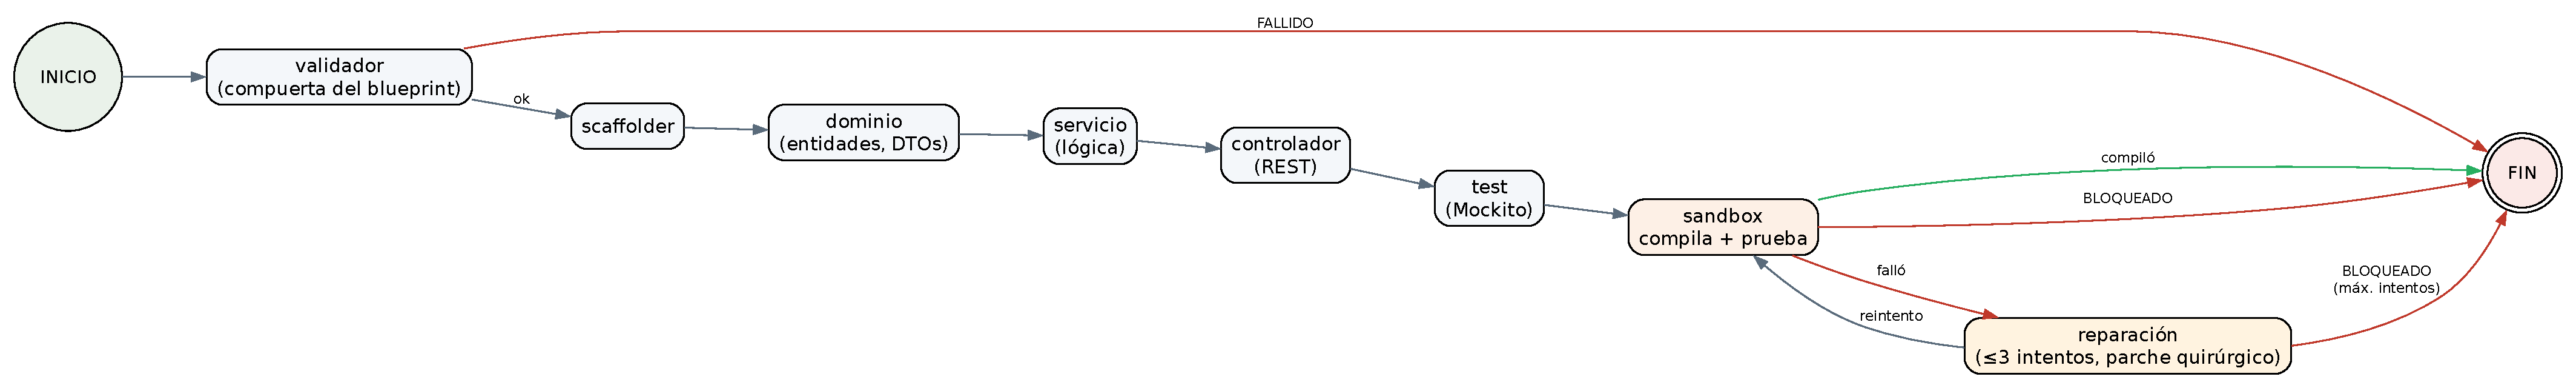
\includegraphics[width=0.9\linewidth]{fig/workflow.pdf}
  \caption{La máquina de estados de generación: columna lineal con un ciclo acotado.}
\end{figure}

Cada agente de modelo recibe, en orden, \emph{el prefijo de habilidad} (hoy vacío),
\emph{el documento de instrucción} (su ``system prompt''), \emph{el payload de la
tarea} (el slice del blueprint y los artefactos previos), \emph{las rutas que posee} y
\emph{el formato de respuesta}. Tres pistas sobre los prompts:

\begin{itemize}[leftmargin=1.4em]
  \item \textbf{Scaffolder}: ``no declares ninguna dependencia fuera de la lista
  blanca'' --- la regla que hace posible la compilación offline.
  \item \textbf{Dominio}: ``los contratos son records nativos; \texttt{@Data} está
  prohibido'' --- inmutabilidad en el borde.
  \item \textbf{Controlador}: ``un \texttt{@RestControllerAdvice} que registra la
  traza'' --- los errores se centralizan y se diagnostican.
  \item \textbf{Test}: ``cada escenario de aceptación se mapea a un método'' --- la
  cobertura sigue a la especificación.
\end{itemize}

\section{El flujo de la aplicación}

El ciclo de vida completo, de especificación a entrega, en diez etapas:

\begin{center}
\begin{tabular}{@{}p{0.30\textwidth}p{0.64\textwidth}@{}}
\toprule
\textbf{Fase} & \textbf{Qué ocurre} \\
\midrule
1. Requisitos & historias BDD y exportación \texttt{spec.md} \\
2. Arquitectura & catálogo de componentes y contratos REST (Mermaid) \\
3. Modelos \& SQL & entidades JPA, DTOs, \texttt{schema.sql}, diagrama ER \\
4. Blueprints & ingesta y validación de \texttt{spec.md} / JSON \\
5. Generación \& Monitor & síntesis autónoma + logs en vivo (SSE) \\
6. Código \& Fix & explorador, tests, diffs de reparación, desbloqueo manual \\
7. Calidad SAST & auditoría, compuerta de calidad, remediación \\
8. DevOps & Dockerfile, compose, CI/CD, k8s, despliegue local \\
9. Entrega & ZIP o publicación Git atómica \\
\bottomrule
\end{tabular}
\end{center}

\section{La interfaz de usuario}

Una aplicación React/Vite de una sola página, diez pestañas en español, tema
claro/oscuro, stepper de ciclo de vida y visores Mermaid para arquitectura y ER. El
panel de configuración LLM permite elegir proveedor (Gemini, Groq, OpenAI, DeepSeek o
mock offline), clave, modelo y verificar la conexión. La interfaz refleja la
verificación honesta de tres estados (verificado / con hallazgos / no evaluable), tras
una auditoría que eliminó varios resultados fabricados.

\section{El coste}

Medido, no estimado, desde el sistema de registro (\texttt{cost\_tracking.db}) y su
espejo MLflow.

\begin{center}
\begin{tabular}{@{}lrrr@{}}
\toprule
\textbf{Alcance} & \textbf{Llamadas} & \textbf{Coste (USD)} & \textbf{Tokens salida} \\
\midrule
Experimento de polaridad & 750 & 6.58 & --- \\
Cinco congelados & 120 & 0.63 & --- \\
Diez difíciles & 50 & 0.64 & --- \\
Sondas / sueltas & $\approx$250 & $\approx$0.16 & --- \\
\midrule
\textbf{Total} & \textbf{1219} & \textbf{8.15} & \textbf{12.48M} \\
\bottomrule
\end{tabular}
\end{center}

\subsection{Uso de tokens (actual, del espejo MLflow y del registro)}

\begin{center}
\begin{tabular}{@{}lrrrr@{}}
\toprule
\textbf{Fuente} & \textbf{Entrada} & \textbf{Salida} & \textbf{Cache} & \textbf{Combinado} \\
\midrule
Registro (autoritativo) & 6.54M & 12.48M & 2.20M & \textbf{19.02M} \\
Espejo MLflow & 5.49M & 9.92M & 1.76M & \textbf{15.41M} \\
\bottomrule
\end{tabular}
\end{center}

Por llamada: $\approx$5{,}360 entrada + $\approx$10{,}240 salida $\approx$ 15.6K tokens; por
servicio (5 llamadas) $\approx$78K tokens. La salida es $\approx$1.9$\times$ la entrada
(esperado: el generador \emph{emite} código). $\approx$2.2M tokens de entrada se
sirvieron desde caché ($\approx$34\%).

Por servicio: \textbf{\$0.052--\$0.077} (diez difíciles), $\approx$\$0.005 por llamada;
por etapa, el test es el más caro (\$0.0061) y dominio el más barato (\$0.0012). Todo
en \texttt{deepseek-flash}.

\begin{notebox}[colframe=warn]
\textbf{El espejo MLflow se ha desviado y puede verse vacío.} El espejo totaliza
\textbf{\$6.39} frente a \textbf{\$8.15} (subestimación del $\approx$22\%) y
\textbf{15.41M} tokens frente a \textbf{19.02M}; además, \texttt{mlflow
ui} abre por defecto el almacén vacío \texttt{mlruns/} en vez de \texttt{mlflow.db}, y
los agregados de sesión (168) cayeron en el experimento legado \texttt{Default}, con 0
en \texttt{agentia}. Hasta reparar el sink, el almacén local es la cifra a citar.
\end{notebox}

\subsection{Datos que faltan y qué hacer}

\begin{itemize}[leftmargin=1.4em]
  \item \textbf{El espejo subestima (20--22\%) y está partido en dos experimentos.}
  \emph{Qué hacer}: arreglar el targeting de experimento en \texttt{mlflow\_sink.py}
  para que los registros de sesión caigan en \texttt{agentia}, y migrar las 877
  ejecuciones legadas de \texttt{Default} (o aceptar que el espejo es solo
  indicativo).
  \item \textbf{Falta desglose por modelo.} Todo es \texttt{deepseek-flash}; para
  comparar proveedores se necesita una corrida con otro modelo. \emph{Qué hacer}:
  una tanda corta (p.\ ej.\ Gemini o Groq) sobre el mismo corpus para tener coste y
  tokens por modelo.
  \item \textbf{El coste de caché es aproximado.} Los tokens cache-hits se registran,
  pero su base de precio no está verificada contra factura. \emph{Qué hacer}: auditar
  \texttt{pricing\_basis} contra la factura del proveedor una vez.
  \item \textbf{Agregados de sesión ausentes en \texttt{agentia}.} \emph{Qué hacer}:
  confirmar que \texttt{mirror\_session\_cost\_record} se invoca al terminar cada
  sesión y escribe \texttt{total\_cost\_usd} en el experimento correcto.
\end{itemize}

\section{Conclusión}

La plataforma pasó de ``no puede verificar su propia salida'' a ``genera, compila y
verifica a \$0.06 por servicio, con una selección guiada por verificación que alcanza
100\% de cobertura con tres candidatos a \$0.20''. El camino que queda es corto y
concreto: \textbf{(1)} hacer determinista el verificador (un montaje), \textbf{(2)}
hacer que la medida pueda moverse (minar fallos de compilación en reglas), y
\textbf{(3)} solo entonces preguntar si un documento de habilidad aporta algo. El
bucle de auto-mejora queda cerrado tras esa compuerta --- que es, literalmente, la
misma compuerta que el diseño siempre exigió.

\end{document}
